%*******************************************************
% Appendix
%*******************************************************
% If problems with the headers: get headings in appendix etc. right
%\markboth{\spacedlowsmallcaps{Appendix}}{\spacedlowsmallcaps{Appendix}}

\chapter{Appenidx}

\section{Mathematica}

\begin{mathematica}[h!]
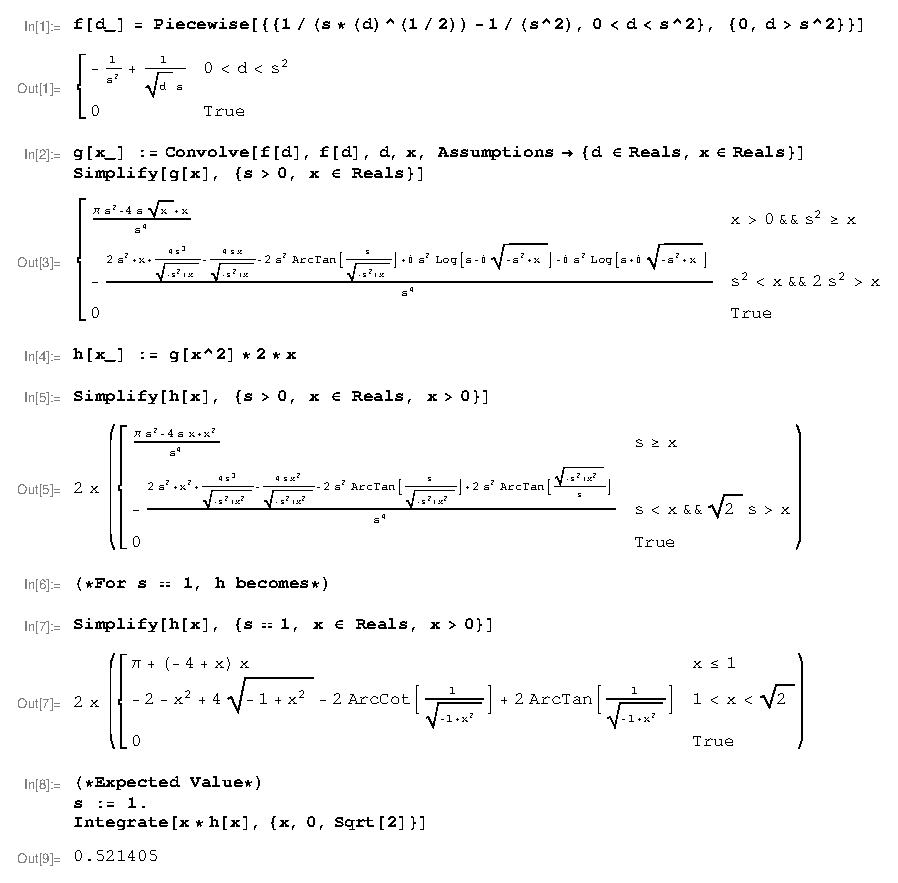
\includegraphics[width=1.2\linewidth, cframe=RoyalBlue 1pt]{mathematica/distance_theorem.pdf}
\caption{some code}
\label{mathematica:distances}
\end{mathematica} 

\begin{remark} Analytic verification that the distribution reported by
  \textcite{Moltchanov2012} in Mathematica.
However the functions behave in the domain numerically equivalent,
shown by 
\end{remark}



% ######################################################################### %
% ------------------------------------------------------------------------- %
%                 Reproducibility in Computational Research         
% ------------------------------------------------------------------------- %
% ######################################################################### %

\section{Reproducibility in Computational Research}\label{sec:reproducibility}

\textcite{Sumatra2012}







%%% Local Variables: 
%%% mode: latex
%%% TeX-master: "../dplths_document"
%%% End: 